% Options for packages loaded elsewhere
\PassOptionsToPackage{unicode}{hyperref}
\PassOptionsToPackage{hyphens}{url}
\PassOptionsToPackage{dvipsnames,svgnames,x11names}{xcolor}
%
\documentclass[
]{article}

\usepackage{amsmath,amssymb}
\usepackage{iftex}
\ifPDFTeX
  \usepackage[T1]{fontenc}
  \usepackage[utf8]{inputenc}
  \usepackage{textcomp} % provide euro and other symbols
\else % if luatex or xetex
  \usepackage{unicode-math}
  \defaultfontfeatures{Scale=MatchLowercase}
  \defaultfontfeatures[\rmfamily]{Ligatures=TeX,Scale=1}
\fi
\usepackage{lmodern}
\ifPDFTeX\else  
    % xetex/luatex font selection
\fi
% Use upquote if available, for straight quotes in verbatim environments
\IfFileExists{upquote.sty}{\usepackage{upquote}}{}
\IfFileExists{microtype.sty}{% use microtype if available
  \usepackage[]{microtype}
  \UseMicrotypeSet[protrusion]{basicmath} % disable protrusion for tt fonts
}{}
\makeatletter
\@ifundefined{KOMAClassName}{% if non-KOMA class
  \IfFileExists{parskip.sty}{%
    \usepackage{parskip}
  }{% else
    \setlength{\parindent}{0pt}
    \setlength{\parskip}{6pt plus 2pt minus 1pt}}
}{% if KOMA class
  \KOMAoptions{parskip=half}}
\makeatother
\usepackage{xcolor}
\setlength{\emergencystretch}{3em} % prevent overfull lines
\setcounter{secnumdepth}{5}
% Make \paragraph and \subparagraph free-standing
\ifx\paragraph\undefined\else
  \let\oldparagraph\paragraph
  \renewcommand{\paragraph}[1]{\oldparagraph{#1}\mbox{}}
\fi
\ifx\subparagraph\undefined\else
  \let\oldsubparagraph\subparagraph
  \renewcommand{\subparagraph}[1]{\oldsubparagraph{#1}\mbox{}}
\fi


\providecommand{\tightlist}{%
  \setlength{\itemsep}{0pt}\setlength{\parskip}{0pt}}\usepackage{longtable,booktabs,array}
\usepackage{calc} % for calculating minipage widths
% Correct order of tables after \paragraph or \subparagraph
\usepackage{etoolbox}
\makeatletter
\patchcmd\longtable{\par}{\if@noskipsec\mbox{}\fi\par}{}{}
\makeatother
% Allow footnotes in longtable head/foot
\IfFileExists{footnotehyper.sty}{\usepackage{footnotehyper}}{\usepackage{footnote}}
\makesavenoteenv{longtable}
\usepackage{graphicx}
\makeatletter
\def\maxwidth{\ifdim\Gin@nat@width>\linewidth\linewidth\else\Gin@nat@width\fi}
\def\maxheight{\ifdim\Gin@nat@height>\textheight\textheight\else\Gin@nat@height\fi}
\makeatother
% Scale images if necessary, so that they will not overflow the page
% margins by default, and it is still possible to overwrite the defaults
% using explicit options in \includegraphics[width, height, ...]{}
\setkeys{Gin}{width=\maxwidth,height=\maxheight,keepaspectratio}
% Set default figure placement to htbp
\makeatletter
\def\fps@figure{htbp}
\makeatother

\usepackage{booktabs}
\usepackage{longtable}
\usepackage{array}
\usepackage{multirow}
\usepackage{wrapfig}
\usepackage{float}
\usepackage{colortbl}
\usepackage{pdflscape}
\usepackage{tabu}
\usepackage{threeparttable}
\usepackage{threeparttablex}
\usepackage[normalem]{ulem}
\usepackage{makecell}
\usepackage{xcolor}
\usepackage{caption}
\usepackage{anyfontsize}
\usepackage{fvextra}
\DefineVerbatimEnvironment{Highlighting}{Verbatim}{breaklines,commandchars=\\\{\}}
\makeatletter
\makeatother
\makeatletter
\makeatother
\makeatletter
\@ifpackageloaded{caption}{}{\usepackage{caption}}
\AtBeginDocument{%
\ifdefined\contentsname
  \renewcommand*\contentsname{Table of contents}
\else
  \newcommand\contentsname{Table of contents}
\fi
\ifdefined\listfigurename
  \renewcommand*\listfigurename{List of Figures}
\else
  \newcommand\listfigurename{List of Figures}
\fi
\ifdefined\listtablename
  \renewcommand*\listtablename{List of Tables}
\else
  \newcommand\listtablename{List of Tables}
\fi
\ifdefined\figurename
  \renewcommand*\figurename{Figure}
\else
  \newcommand\figurename{Figure}
\fi
\ifdefined\tablename
  \renewcommand*\tablename{Table}
\else
  \newcommand\tablename{Table}
\fi
}
\@ifpackageloaded{float}{}{\usepackage{float}}
\floatstyle{ruled}
\@ifundefined{c@chapter}{\newfloat{codelisting}{h}{lop}}{\newfloat{codelisting}{h}{lop}[chapter]}
\floatname{codelisting}{Listing}
\newcommand*\listoflistings{\listof{codelisting}{List of Listings}}
\makeatother
\makeatletter
\@ifpackageloaded{caption}{}{\usepackage{caption}}
\@ifpackageloaded{subcaption}{}{\usepackage{subcaption}}
\makeatother
\makeatletter
\@ifpackageloaded{tcolorbox}{}{\usepackage[skins,breakable]{tcolorbox}}
\makeatother
\makeatletter
\@ifundefined{shadecolor}{\definecolor{shadecolor}{rgb}{.97, .97, .97}}
\makeatother
\makeatletter
\makeatother
\makeatletter
\makeatother
\ifLuaTeX
  \usepackage{selnolig}  % disable illegal ligatures
\fi
\IfFileExists{bookmark.sty}{\usepackage{bookmark}}{\usepackage{hyperref}}
\IfFileExists{xurl.sty}{\usepackage{xurl}}{} % add URL line breaks if available
\urlstyle{same} % disable monospaced font for URLs
\hypersetup{
  pdftitle={BioMADE Experiment: Definition Complexity and Issue},
  colorlinks=true,
  linkcolor={blue},
  filecolor={Maroon},
  citecolor={Blue},
  urlcolor={Blue},
  pdfcreator={LaTeX via pandoc}}

\title{BioMADE Experiment: Definition Complexity and Issue}
\author{}
\date{}

\begin{document}
\maketitle
\RecustomVerbatimEnvironment{verbatim}{Verbatim}{
showspaces = false,
showtabs = false,
breaksymbolleft={},
breaklines
}

\ifdefined\Shaded\renewenvironment{Shaded}{\begin{tcolorbox}[boxrule=0pt, interior hidden, borderline west={3pt}{0pt}{shadecolor}, enhanced, breakable, frame hidden, sharp corners]}{\end{tcolorbox}}\fi

Data were collected by Qualtrics between August 29 and September 13,
2025. Of the final sample of 1,754, Qualtrics designated 1,190 responses
as ``good completes.''

The table below shows demographic information by experimental
condition--none of the differences in the demographics between
conditions are significant, which is indicative of random assignment to
the experimental conditions.

\begin{table}
\fontsize{12.0pt}{14.4pt}\selectfont
\begin{tabular*}{\linewidth}{@{\extracolsep{\fill}}lc}
\toprule
\textbf{Characteristic} & \textbf{N = 1,190}\textsuperscript{\textit{1}} \\ 
\midrule\addlinespace[2.5pt]
Age & 48 (17) \\ 
Gender &  \\ 
    male & 48\% \\ 
    female & 52\% \\ 
Race (Non-White/White) &  \\ 
    non-white & 26\% \\ 
    white & 74\% \\ 
Education &  \\ 
    Less than high school & 7.0\% \\ 
    High school graduate & 55\% \\ 
    Some college & 38\% \\ 
    2-year degree & 0\% \\ 
    4-year degree & 0\% \\ 
    Post-graduate degree & 0\% \\ 
Income &  \\ 
    Less than \$25,000 & 20\% \\ 
    \$25,000 to \$49,999 & 25\% \\ 
    \$50,000 to \$74,999 & 19\% \\ 
    \$75,000 to \$99,999 & 11\% \\ 
    \$100,000 to \$124,999 & 8.2\% \\ 
    \$125,000 to \$149,999 & 7.9\% \\ 
    \$150,000 to \$174,999 & 4.2\% \\ 
    \$175,000 to \$199,999 & 1.9\% \\ 
    \$200,000 or more & 3.1\% \\ 
\bottomrule
\end{tabular*}
\begin{minipage}{\linewidth}
\textsuperscript{\textit{1}}Mean (SD); \%\\
\end{minipage}
\end{table}

\hypertarget{manipulation-checks}{%
\section{Manipulation Checks}\label{manipulation-checks}}

\hypertarget{perceived-difficulty-of-self-understanding-provided-definition}{%
\subsection{Perceived difficulty of self-understanding provided
definition}\label{perceived-difficulty-of-self-understanding-provided-definition}}

The first manipulation check is a question about the perceived
difficulty (be the respondent) of understanding the definition provided
in the survey. The figure below shows mean levels of perceived
difficulty of understanding the definition provided in the survey by
simple vs.~complex definition. The difference in mean levels of
perceived difficulty was significant between the conditions
(\(t = -2.67\), \(p = .008\)).

\begin{figure}

{\centering 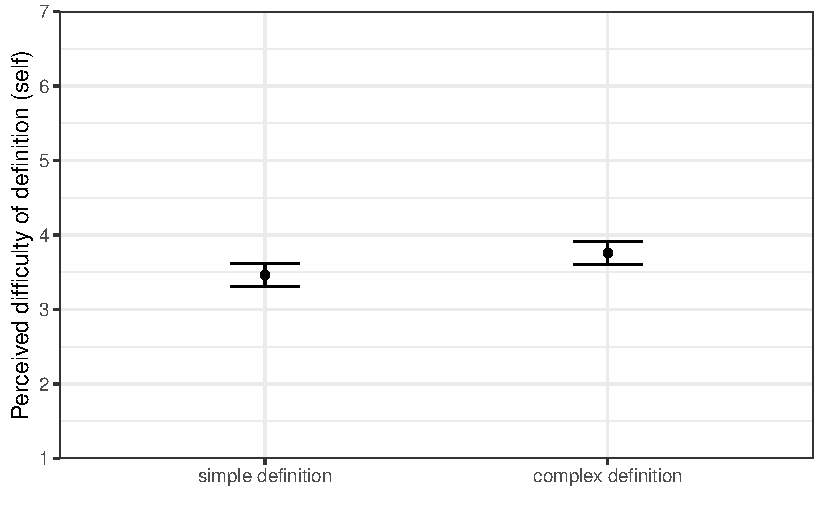
\includegraphics{BioMADE-fall2025-data-analysis_files/figure-pdf/defn-MC-self-1.pdf}

}

\end{figure}

\hypertarget{perceived-difficulty-of-other-understanding-provided-definition}{%
\subsection{Perceived difficulty of other-understanding provided
definition}\label{perceived-difficulty-of-other-understanding-provided-definition}}

The second manipulation check question asked respondents about their
perceptions of how difficult it might be for others to understand the
provided definition. The figure below shows mean levels of perceived
difficulty that others might have understanding the definitions provided
in the survey. The difference in mean levels of perceived difficulty was
significant between the conditions (\(t = -3.13\), \(p = .002\)).

\begin{figure}

{\centering 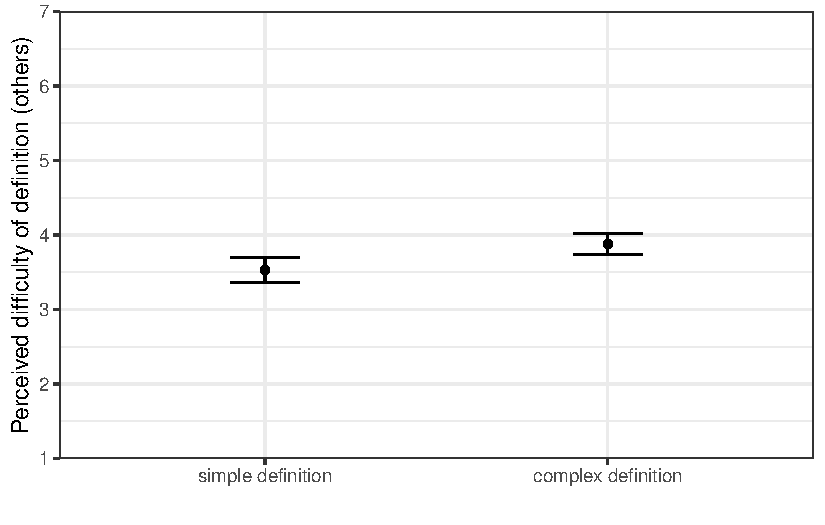
\includegraphics{BioMADE-fall2025-data-analysis_files/figure-pdf/defn-MC-other-1.pdf}

}

\end{figure}

I was not sure what to do with the question about the terms used in the
definition or the open-ended questions, which require coding.

\hypertarget{dependent-variables}{%
\section{Dependent Variables}\label{dependent-variables}}

\hypertarget{curiosity}{%
\subsection{Curiosity}\label{curiosity}}

Created a variable from the items measuring curiosity in each of the
experimental conditions (\texttt{Q29\_1}: \texttt{Q29\_4},
\texttt{Q44\_1}:\texttt{Q44\_4}, \texttt{Q59\_1}:\texttt{Q59\_4},
\texttt{Q74\_1}:\texttt{Q74\_4}). The table below shows the means and
standard deviations for this variable in the whole sample, as well as in
the four experimental conditions. Analysis of variance (ANOVA) reveals
no significant differences in the mean of curiosity between the
conditions (\(F(3, 1185) = 0.34\), \(p = .80\)).

\begin{figure}

{\centering 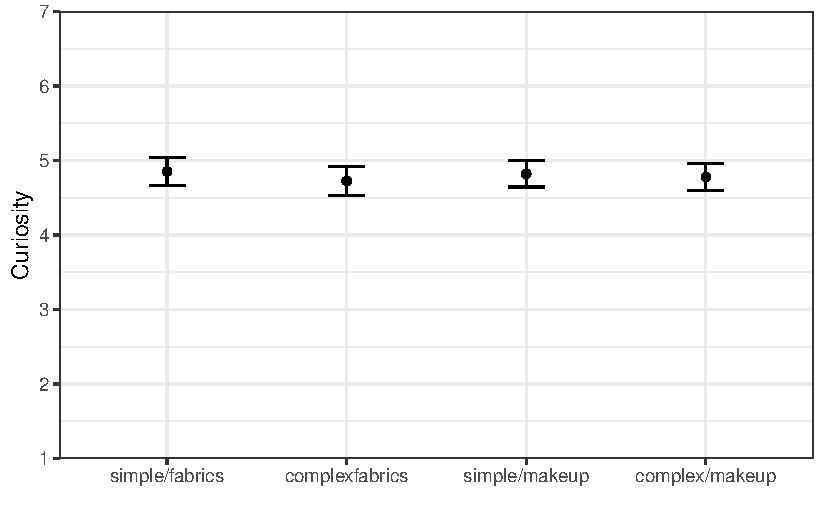
\includegraphics{BioMADE-fall2025-data-analysis_files/figure-pdf/curious-1.pdf}

}

\end{figure}

\hypertarget{information-seeking}{%
\subsection{Information Seeking}\label{information-seeking}}

Created a variable from the items measuring intentions to seek
information in each of the experimental conditions (\texttt{Q30\_1}:
\texttt{Q30\_5}, \texttt{Q45\_1}:\texttt{Q45\_5},
\texttt{Q60\_1}:\texttt{Q60\_5}, \texttt{Q75\_1}:\texttt{Q75\_5}). The
table below shows the means and standard deviations for this variable in
the whole sample, as well as in the four experimental conditions. There
were no significant differences in this outcome variable by experimental
condition (\(F(3, 1186) = .51\), \(p = .68\)).

\begin{figure}

{\centering 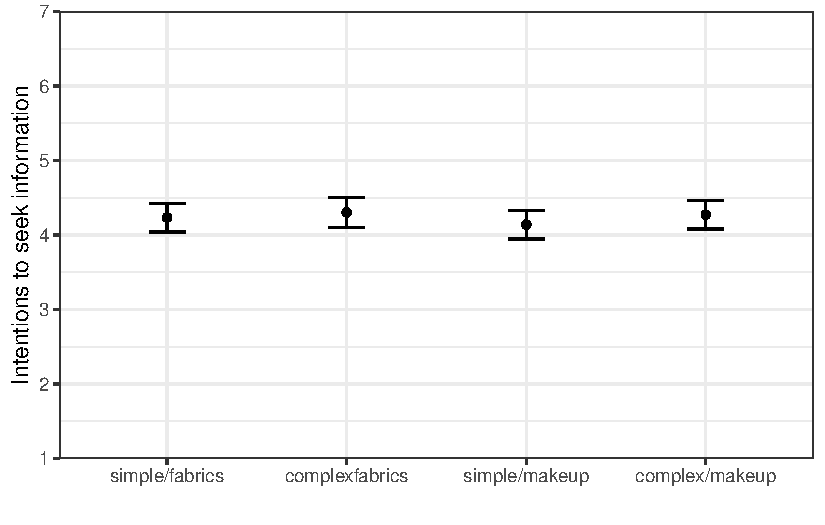
\includegraphics{BioMADE-fall2025-data-analysis_files/figure-pdf/infoseek-1.pdf}

}

\end{figure}

\hypertarget{support-for-biomanufacturing-federal-and-state-funding-of-research}{%
\subsection{Support for Biomanufacturing, Federal and State Funding of
Research}\label{support-for-biomanufacturing-federal-and-state-funding-of-research}}

Created a variable from the items measuring intentions to seek
information in each of the experimental conditions (\texttt{Q31\_1}:
\texttt{Q31\_3}, \texttt{Q46\_1}:\texttt{Q46\_3},
\texttt{Q61\_1}:\texttt{Q61\_3}, \texttt{Q76\_1}:\texttt{Q76\_3}). The
table below shows the means and standard deviations for this variable in
the whole sample, as well as in the four experimental conditions. There
were no significant differences in the means of support by experimental
condition (\(F(3, 1186) = .75\), \(p = .53\)).

Even though the factor analysis revealed a single factor for this
variable, it might be worth considering (for content validity)
separating general support for biomanufacturing and support for funding
(state and federal) of biomanufacturing research.

\begin{figure}

{\centering 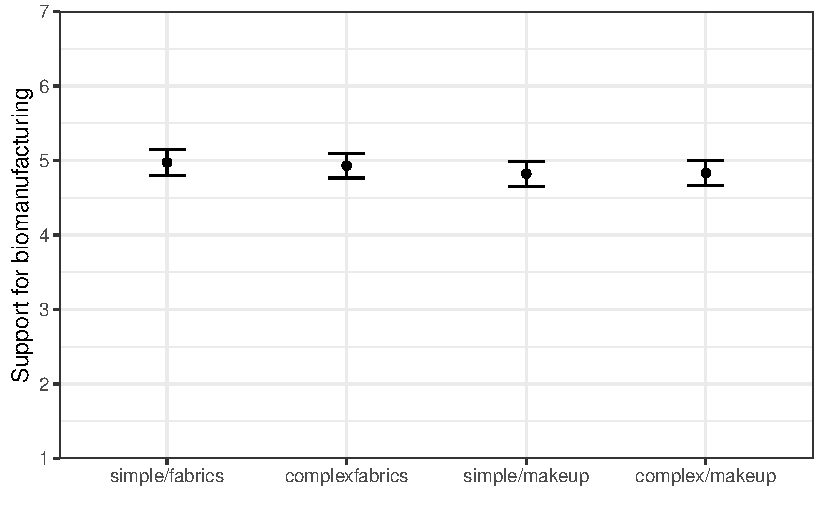
\includegraphics{BioMADE-fall2025-data-analysis_files/figure-pdf/support-1.pdf}

}

\end{figure}

\hypertarget{risks-and-benefits}{%
\subsection{Risks and Benefits}\label{risks-and-benefits}}

Created a variable from the single items each measuring risk and benefit
perceptions in each of the experimental conditions (\texttt{Q31\_4},
\texttt{Q31\_5}, \texttt{Q46\_4}, \texttt{Q46\_5}, \texttt{Q61\_4},
\texttt{Q61\_5}, \texttt{Q76\_4}, \texttt{Q76\_5}). The table below
shows the means and standard deviations for this variable in the whole
sample, as well as in the four experimental conditions. There were no
significant differences in perceived benefits between conditions
(\(F(3, 1183) = .19\), \(p = .90\)). However, there were significant
differences in risk perceptions by experimental conditions
(\(F(3,1186) = 3.27\), \(p = .02\)).

\begin{figure}

{\centering 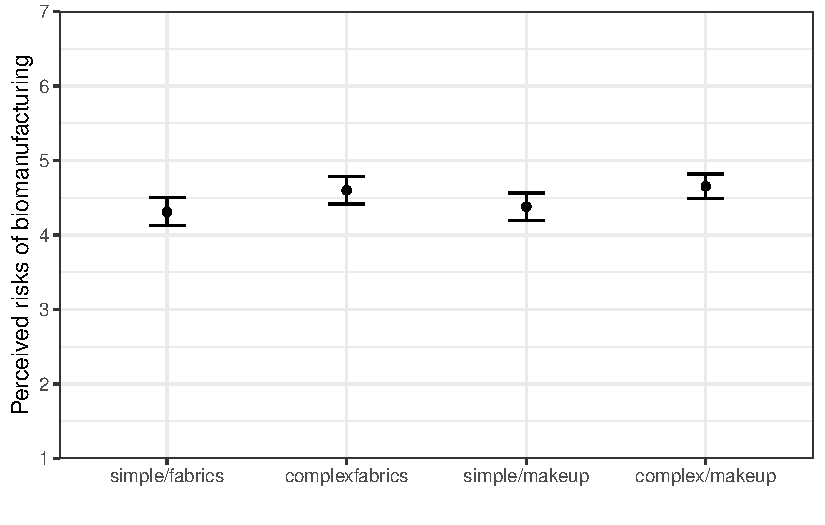
\includegraphics{BioMADE-fall2025-data-analysis_files/figure-pdf/risks-1.pdf}

}

\end{figure}

\begin{figure}

{\centering 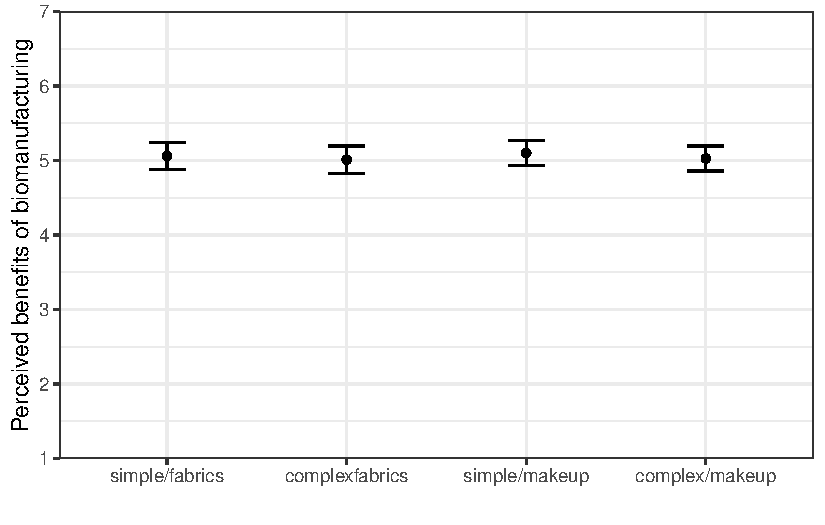
\includegraphics{BioMADE-fall2025-data-analysis_files/figure-pdf/benefits-1.pdf}

}

\end{figure}



\end{document}
